\textbf{Ejercicio 4.} (25 pts.) Realiza la inferencia de tipos vista en clase sobre la siguiente expresión, recuerda obtener las restricciones y usar el algoritmo de unificación para resolverlas. \vspace{0.3cm}

\begin{lstlisting}
((lambda (x) (* x 2)) (+ 2 3))
\end{lstlisting}

\textbf{Obtener las subexpresiones} \vspace{0.3cm}

\begin{itemize}
    \item 1. \hl{((lambda (x) (* x 2)) (+ 2 3))}
    \item 2. (\hl{(lambda (x) (* x 2))} (+ 2 3))
    \item 3. ((lambda \hl{(x)} (* x 2)) (+ 2 3))
    \item 4. ((lambda (x) \hl{(* x 2)}) (+ 2 3))
    \item 5. ((lambda (x) (* \hl{x} 2)) (+ 2 3))
    \item 6. ((lambda (x) (* x \hl{2})) (+ 2 3))
    \item 7. ((lambda (x) (* x 2)) \hl{(+ 2 3)})
    \item 8. ((lambda (x) (* x 2)) (+ \hl{2} 3))
    \item 9. ((lambda (x) (* x 2)) (+ 2 \hl{3}))
\end{itemize}

\textbf{Obtener las restricciones}
\begin{align*}
    [[2]] &= [[7]] \rightarrow [[1]] \\
    [[2]] &= [[3]] \rightarrow [[4]] \\
    [[3]] &= [[5]] \\ 
    [[4]] &= number \\
    [[5]] &= number \\
    [[6]] &= number \\
    [[7]] &= number \\
    [[8]] &= number \\
    [[9]] &= number
\end{align*}

\textbf{Sustituir en las restricciones (algoritmo de unificación)} \vspace{0.3cm}

\begin{center}
    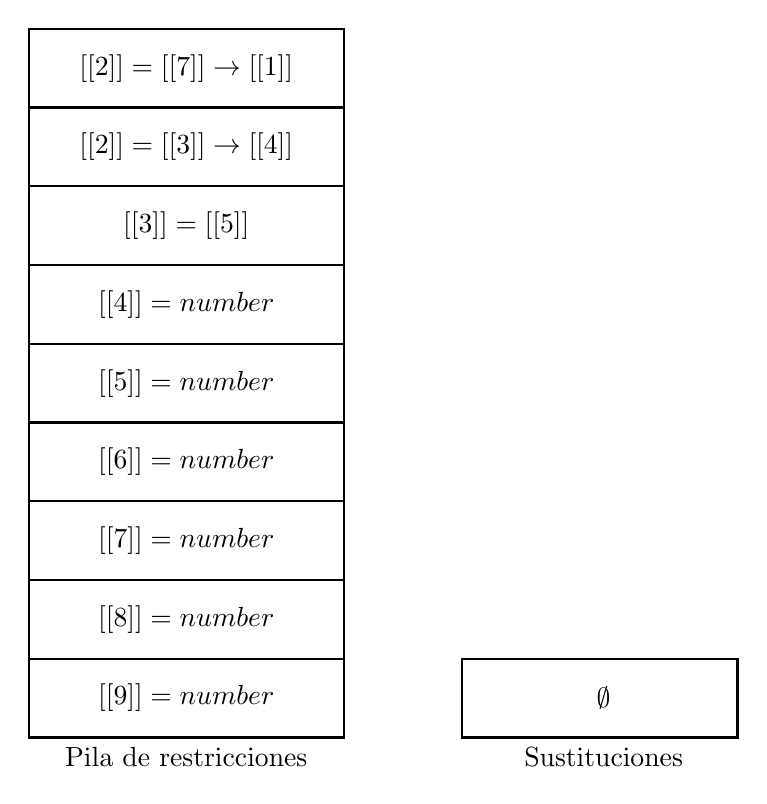
\begin{tikzpicture}
        % Pila 1
        \foreach \y/\val in {
            0/$[[9]] = number$,
            1/$[[8]] = number$,
            2/$[[7]] = number$,
            3/$[[6]] = number$,
            4/$[[5]] = number$,
            5/$[[4]] = number$, 
            6/$[[3]] = [[5]]$, 
            7/$[[2]] = [[3]] \rightarrow [[4]]$, 
            8/$[[2]] = [[7]] \rightarrow [[1]]$
            } {
            \draw[thick] (-1.5, \y) rectangle (2.5, \y+1);
            \node at (0.5, \y+0.5) {\val};
        }
        \node[below] at (0.5, 0) {Pila de restricciones};
    
        % Pila 2
        \foreach \y/\val in {0/$\emptyset$} {
            \draw[thick] (4, \y) rectangle (7.5, \y+1);
            \node at (5.8, \y+0.5) {\val};
        }
        \node[below] at (5.8, 0) {Sustituciones};
    \end{tikzpicture}
\end{center}

\begin{center}
    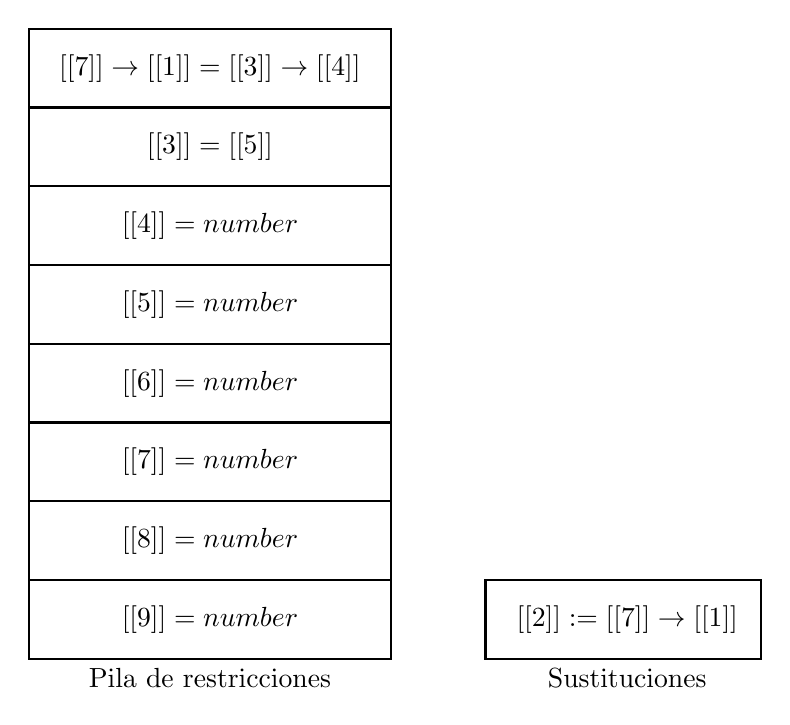
\begin{tikzpicture}
        % Pila 1
        \foreach \y/\val in {
            0/$[[9]] = number$,
            1/$[[8]] = number$,
            2/$[[7]] = number$,
            3/$[[6]] = number$,
            4/$[[5]] = number$,
            5/$[[4]] = number$, 
            6/$[[3]] = [[5]]$, 
            7/$[[7]] \rightarrow [[1]] = [[3]] \rightarrow [[4]]$, 
            } {
            \draw[thick] (-1.8, \y) rectangle (2.8, \y+1);
            \node at (0.5, \y+0.5) {\val};
        }
        \node[below] at (0.5, 0) {Pila de restricciones};
    
        % Pila 2
        \foreach \y/\val in {0/$[[2]] := [[7]] \rightarrow [[1]]$} {
            \draw[thick] (4, \y) rectangle (7.5, \y+1);
            \node at (5.8, \y+0.5) {\val};
        }
        \node[below] at (5.8, 0) {Sustituciones};
    \end{tikzpicture}
\end{center}

\begin{center}
    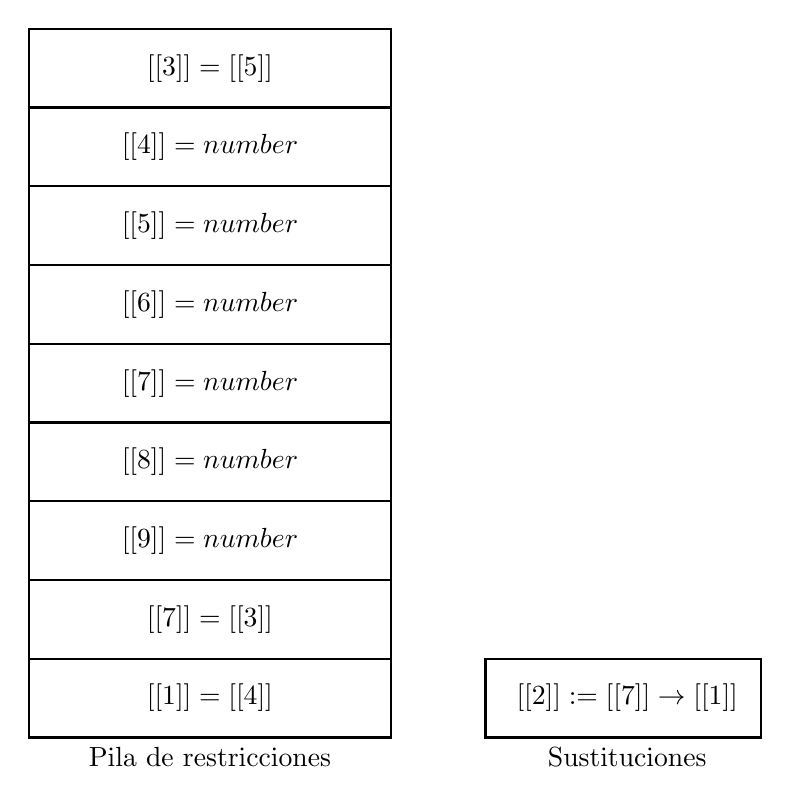
\begin{tikzpicture}
        % Pila 1
        \foreach \y/\val in {
            0/$[[1]] = [[4]]$,
            1/$[[7]] = [[3]]$,
            2/$[[9]] = number$,
            3/$[[8]] = number$,
            4/$[[7]] = number$,
            5/$[[6]] = number$,
            6/$[[5]] = number$,
            7/$[[4]] = number$, 
            8/$[[3]] = [[5]]$,  
            } {
            \draw[thick] (-1.8, \y) rectangle (2.8, \y+1);
            \node at (0.5, \y+0.5) {\val};
        }
        \node[below] at (0.5, 0) {Pila de restricciones};
    
        % Pila 2
        \foreach \y/\val in {
            0/$[[2]] := [[7]] \rightarrow [[1]]$
        } {
            \draw[thick] (4, \y) rectangle (7.5, \y+1);
            \node at (5.8, \y+0.5) {\val};
        }
        \node[below] at (5.8, 0) {Sustituciones};
    \end{tikzpicture}
\end{center}

\begin{center}
    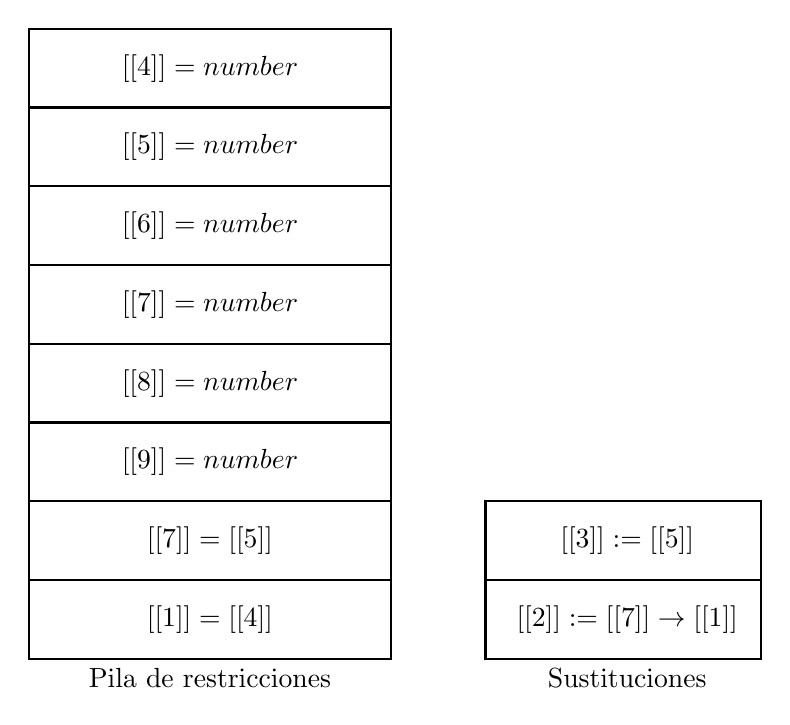
\begin{tikzpicture}
        % Pila 1
        \foreach \y/\val in {
            0/$[[1]] = [[4]]$,
            1/$[[7]] = [[5]]$,
            2/$[[9]] = number$,
            3/$[[8]] = number$,
            4/$[[7]] = number$,
            5/$[[6]] = number$,
            6/$[[5]] = number$,
            7/$[[4]] = number$, 
            } {
            \draw[thick] (-1.8, \y) rectangle (2.8, \y+1);
            \node at (0.5, \y+0.5) {\val};
        }
        \node[below] at (0.5, 0) {Pila de restricciones};
    
        % Pila 2
        \foreach \y/\val in {
            0/$[[2]] := [[7]] \rightarrow [[1]]$,
            1/$[[3]] := [[5]]$
        } {
            \draw[thick] (4, \y) rectangle (7.5, \y+1);
            \node at (5.8, \y+0.5) {\val};
        }
        \node[below] at (5.8, 0) {Sustituciones};
    \end{tikzpicture}
\end{center}

\begin{center}
    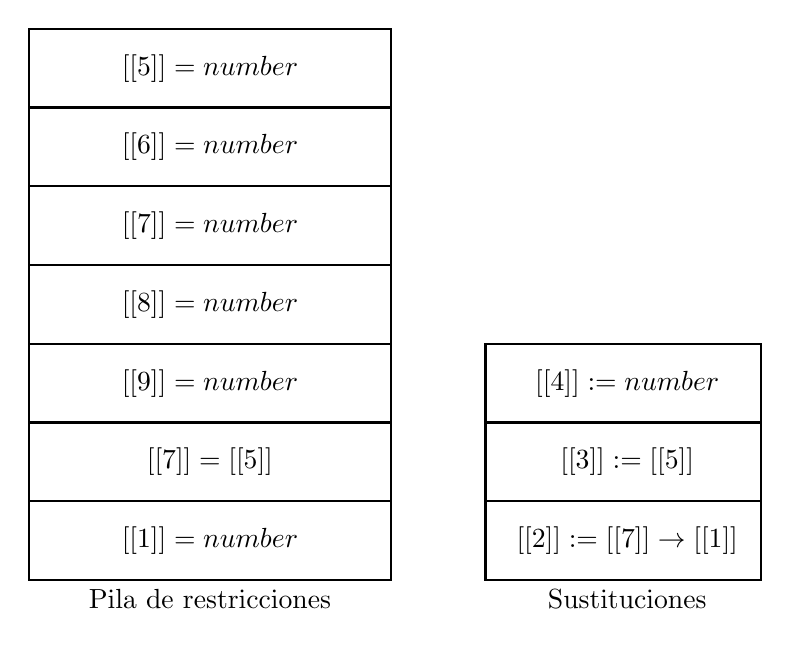
\begin{tikzpicture}
        % Pila 1
        \foreach \y/\val in {
            0/$[[1]] = number$,
            1/$[[7]] = [[5]]$,
            2/$[[9]] = number$,
            3/$[[8]] = number$,
            4/$[[7]] = number$,
            5/$[[6]] = number$,
            6/$[[5]] = number$,
            } {
            \draw[thick] (-1.8, \y) rectangle (2.8, \y+1);
            \node at (0.5, \y+0.5) {\val};
        }
        \node[below] at (0.5, 0) {Pila de restricciones};
    
        % Pila 2
        \foreach \y/\val in {
            0/$[[2]] := [[7]] \rightarrow [[1]]$,
            1/$[[3]] := [[5]]$,
            2/$[[4]] := number$
        } {
            \draw[thick] (4, \y) rectangle (7.5, \y+1);
            \node at (5.8, \y+0.5) {\val};
        }
        \node[below] at (5.8, 0) {Sustituciones};
    \end{tikzpicture}
\end{center}

\begin{center}
    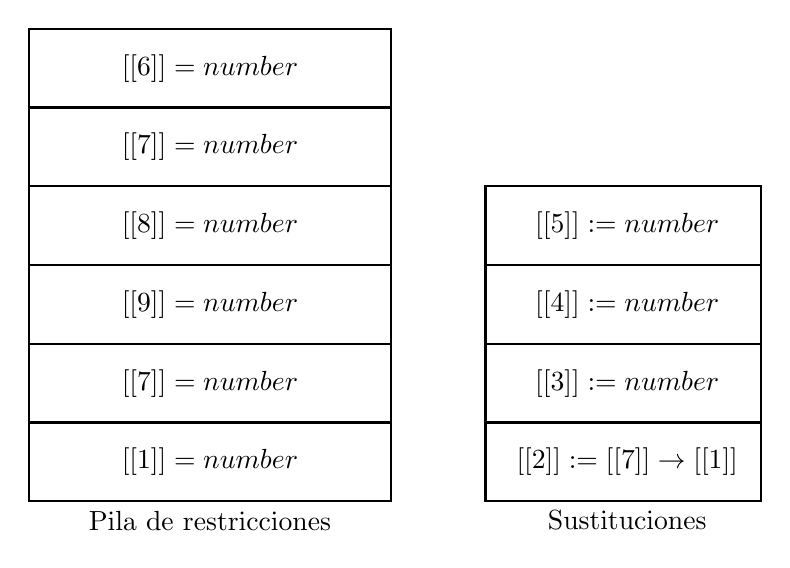
\begin{tikzpicture}
        % Pila 1
        \foreach \y/\val in {
            0/$[[1]] = number$,
            1/$[[7]] = number$,
            2/$[[9]] = number$,
            3/$[[8]] = number$,
            4/$[[7]] = number$,
            5/$[[6]] = number$,
            } {
            \draw[thick] (-1.8, \y) rectangle (2.8, \y+1);
            \node at (0.5, \y+0.5) {\val};
        }
        \node[below] at (0.5, 0) {Pila de restricciones};
    
        % Pila 2
        \foreach \y/\val in {
            0/$[[2]] := [[7]] \rightarrow [[1]]$,
            1/$[[3]] := number$,
            2/$[[4]] := number$,
            3/$[[5]] := number$
        } {
            \draw[thick] (4, \y) rectangle (7.5, \y+1);
            \node at (5.8, \y+0.5) {\val};
        }
        \node[below] at (5.8, 0) {Sustituciones};
    \end{tikzpicture}
\end{center}

\begin{center}
    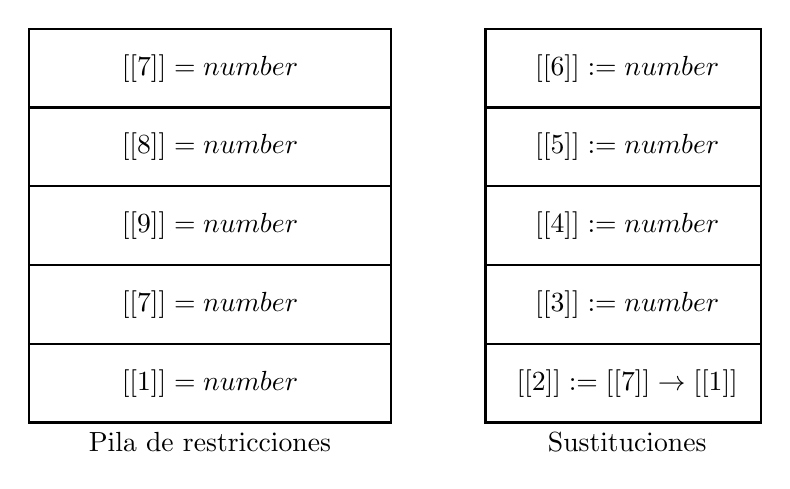
\begin{tikzpicture}
        % Pila 1
        \foreach \y/\val in {
            0/$[[1]] = number$,
            1/$[[7]] = number$,
            2/$[[9]] = number$,
            3/$[[8]] = number$,
            4/$[[7]] = number$,
            } {
            \draw[thick] (-1.8, \y) rectangle (2.8, \y+1);
            \node at (0.5, \y+0.5) {\val};
        }
        \node[below] at (0.5, 0) {Pila de restricciones};
    
        % Pila 2
        \foreach \y/\val in {
            0/$[[2]] := [[7]] \rightarrow [[1]]$,
            1/$[[3]] := number$,
            2/$[[4]] := number$,
            3/$[[5]] := number$,
            4/$[[6]] := number$
        } {
            \draw[thick] (4, \y) rectangle (7.5, \y+1);
            \node at (5.8, \y+0.5) {\val};
        }
        \node[below] at (5.8, 0) {Sustituciones};
    \end{tikzpicture}
\end{center}

\begin{center}
    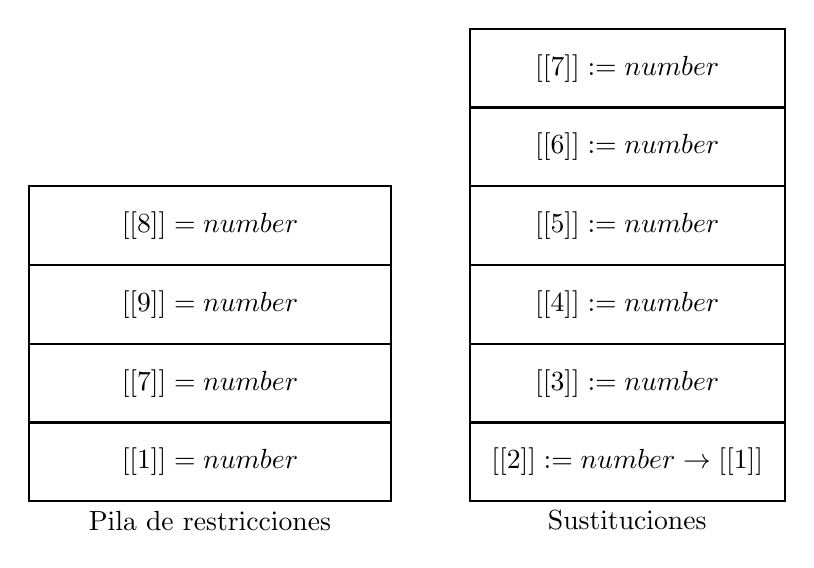
\begin{tikzpicture}
        % Pila 1
        \foreach \y/\val in {
            0/$[[1]] = number$,
            1/$[[7]] = number$,
            2/$[[9]] = number$,
            3/$[[8]] = number$,
            } {
            \draw[thick] (-1.8, \y) rectangle (2.8, \y+1);
            \node at (0.5, \y+0.5) {\val};
        }
        \node[below] at (0.5, 0) {Pila de restricciones};
    
        % Pila 2
        \foreach \y/\val in {
            0/$[[2]] := number \rightarrow [[1]]$,
            1/$[[3]] := number$,
            2/$[[4]] := number$,
            3/$[[5]] := number$,
            4/$[[6]] := number$,
            5/$[[7]] := number$
        } {
            \draw[thick] (3.8, \y) rectangle (7.8, \y+1);
            \node at (5.8, \y+0.5) {\val};
        }
        \node[below] at (5.8, 0) {Sustituciones};
    \end{tikzpicture}
\end{center}

\begin{center}
    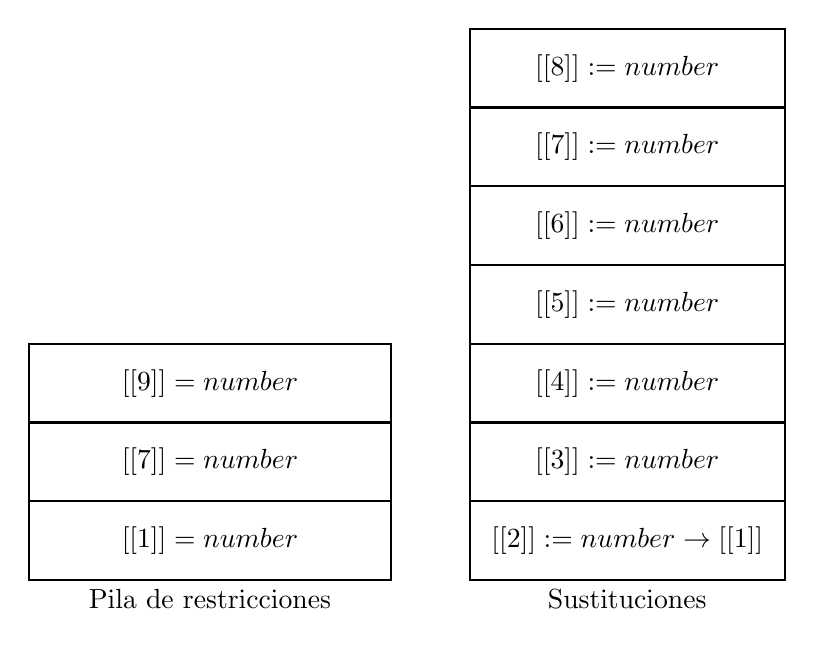
\begin{tikzpicture}
        % Pila 1
        \foreach \y/\val in {
            0/$[[1]] = number$,
            1/$[[7]] = number$,
            2/$[[9]] = number$,
            } {
            \draw[thick] (-1.8, \y) rectangle (2.8, \y+1);
            \node at (0.5, \y+0.5) {\val};
        }
        \node[below] at (0.5, 0) {Pila de restricciones};
    
        % Pila 2
        \foreach \y/\val in {
            0/$[[2]] := number \rightarrow [[1]]$,
            1/$[[3]] := number$,
            2/$[[4]] := number$,
            3/$[[5]] := number$,
            4/$[[6]] := number$,
            5/$[[7]] := number$,
            6/$[[8]] := number$
        } {
            \draw[thick] (3.8, \y) rectangle (7.8, \y+1);
            \node at (5.8, \y+0.5) {\val};
        }
        \node[below] at (5.8, 0) {Sustituciones};
    \end{tikzpicture}
\end{center}

\begin{center}
    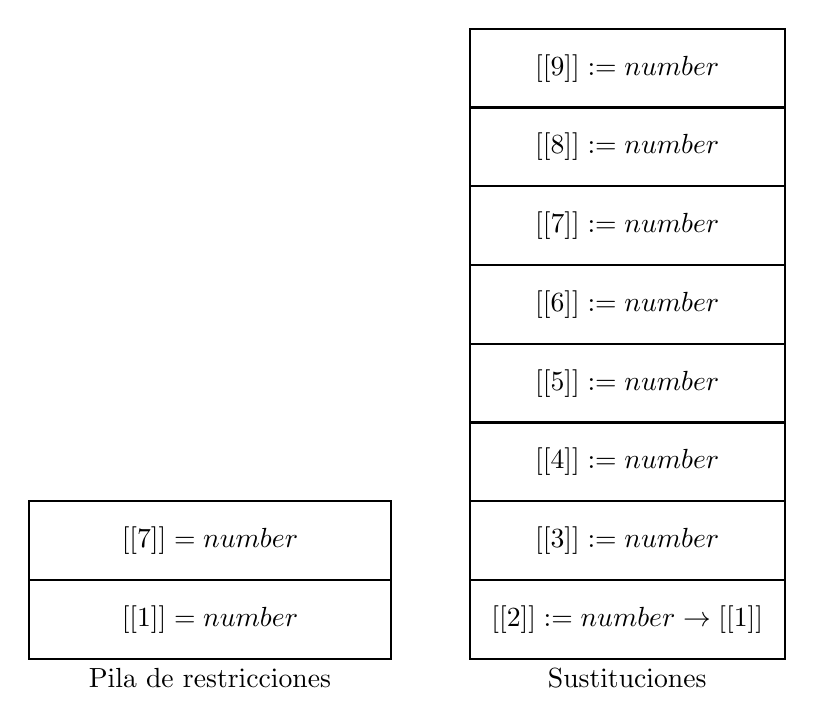
\begin{tikzpicture}
        % Pila 1
        \foreach \y/\val in {
            0/$[[1]] = number$,
            1/$[[7]] = number$,
            } {
            \draw[thick] (-1.8, \y) rectangle (2.8, \y+1);
            \node at (0.5, \y+0.5) {\val};
        }
        \node[below] at (0.5, 0) {Pila de restricciones};
    
        % Pila 2
        \foreach \y/\val in {
            0/$[[2]] := number \rightarrow [[1]]$,
            1/$[[3]] := number$,
            2/$[[4]] := number$,
            3/$[[5]] := number$,
            4/$[[6]] := number$,
            5/$[[7]] := number$,
            6/$[[8]] := number$,
            7/$[[9]] := number$
        } {
            \draw[thick] (3.8, \y) rectangle (7.8, \y+1);
            \node at (5.8, \y+0.5) {\val};
        }
        \node[below] at (5.8, 0) {Sustituciones};
    \end{tikzpicture}
\end{center}

\begin{center}
    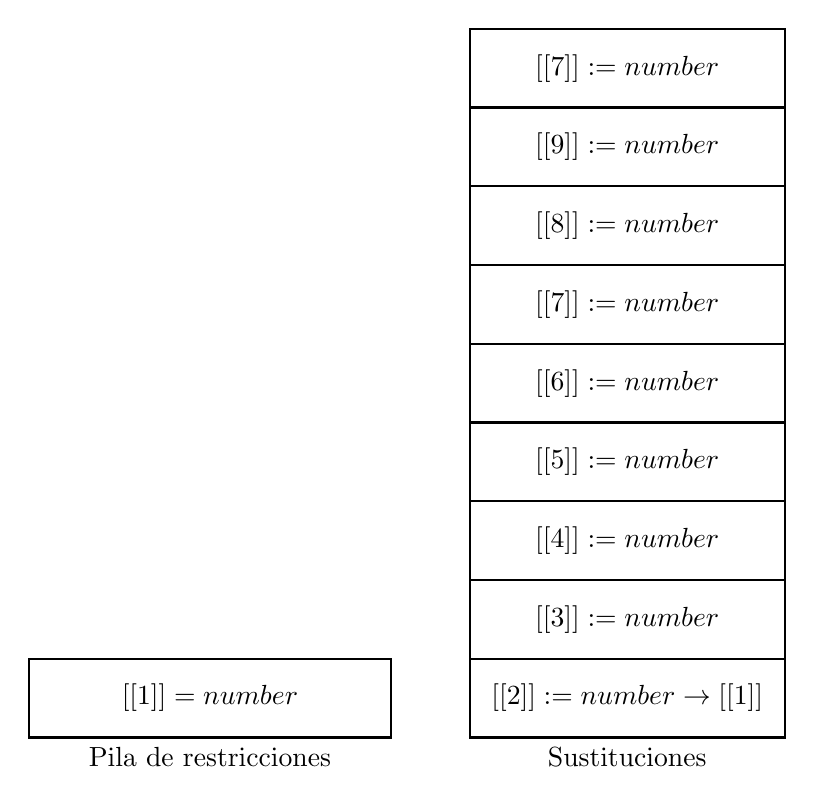
\begin{tikzpicture}
        % Pila 1
        \foreach \y/\val in {
            0/$[[1]] = number$,
            } {
            \draw[thick] (-1.8, \y) rectangle (2.8, \y+1);
            \node at (0.5, \y+0.5) {\val};
        }
        \node[below] at (0.5, 0) {Pila de restricciones};
    
        % Pila 2
        \foreach \y/\val in {
            0/$[[2]] := number \rightarrow [[1]]$,
            1/$[[3]] := number$,
            2/$[[4]] := number$,
            3/$[[5]] := number$,
            4/$[[6]] := number$,
            5/$[[7]] := number$,
            6/$[[8]] := number$,
            7/$[[9]] := number$,
            8/$[[7]] := number$,
        } {
            \draw[thick] (3.8, \y) rectangle (7.8, \y+1);
            \node at (5.8, \y+0.5) {\val};
        }
        \node[below] at (5.8, 0) {Sustituciones};
    \end{tikzpicture}
\end{center}

\begin{center}
    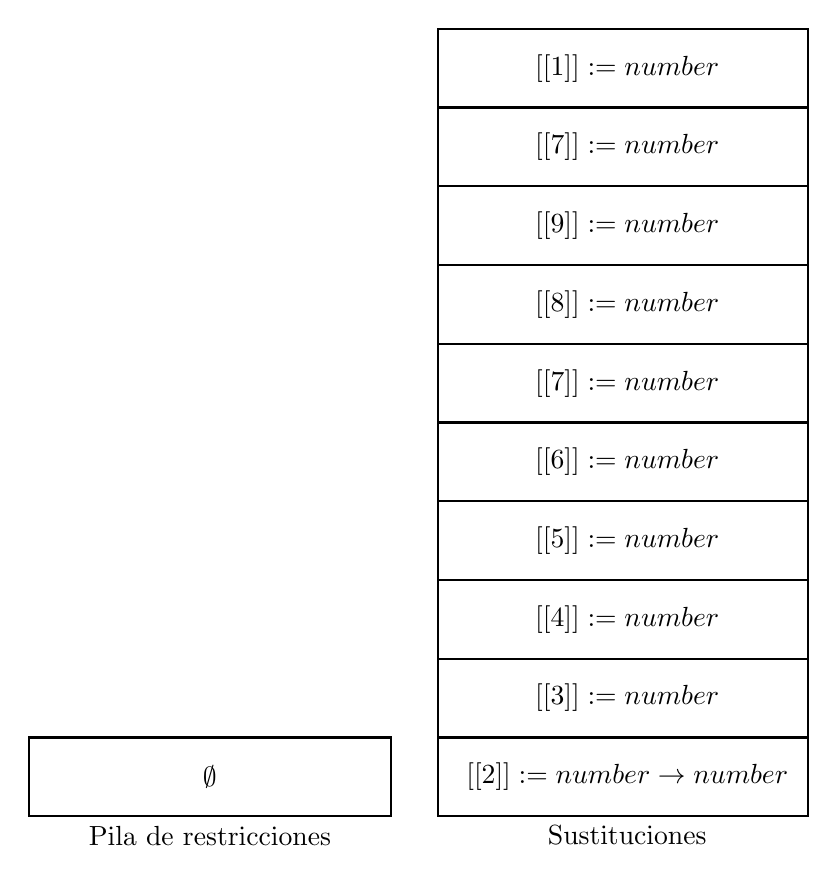
\begin{tikzpicture}
        % Pila 1
        \foreach \y/\val in {
            0/$\emptyset$,
            } {
            \draw[thick] (-1.8, \y) rectangle (2.8, \y+1);
            \node at (0.5, \y+0.5) {\val};
        }
        \node[below] at (0.5, 0) {Pila de restricciones};
    
        % Pila 2
        \foreach \y/\val in {
            0/$[[2]] := number \rightarrow number$,
            1/$[[3]] := number$,
            2/$[[4]] := number$,
            3/$[[5]] := number$,
            4/$[[6]] := number$,
            5/$[[7]] := number$,
            6/$[[8]] := number$,
            7/$[[9]] := number$,
            8/$[[7]] := number$,
            9/$[[1]] := number$
        } {
            \draw[thick] (3.4, \y) rectangle (8.1, \y+1);
            \node at (5.8, \y+0.5) {\val};
        }
        \node[below] at (5.8, 0) {Sustituciones};
    \end{tikzpicture}
\end{center}

Que tiene sentido pues la expresión original era una aplicación que usaba la función que va de $number \rightarrow number$ y el argumento es una suma de tipo $number$ el cuerpo de la función nos regresa efectivamente un number siempre y cuando x sea un número. \vspace{0.3cm}